\documentclass{article}

\usepackage{amsmath,amssymb,amsthm,bm}
\usepackage{graphicx}
\usepackage{subcaption}
\usepackage{float}
\usepackage{xifthen}
\usepackage{hyperref}
\hypersetup{
    colorlinks=true,
    linkcolor=blue,
    %filecolor=magenta,
    urlcolor=cyan
}

\newcommand{\der}[3][1]{
	\frac{{\text{d}^{
		\ifthenelse{\equal{#1}{1}}{}{\,#1}
	}
	{#2} }}
	{\text{d} {#3}^{
		\ifthenelse{\equal{#1}{1}}{}{#1}
	}
	}
}

\newcommand{\pder}[3][1]{
	\frac{{\partial^{
		\ifthenelse{\equal{#1}{1}}{}{\,#1}
	}
	{#2}}}
	{\partial {#3}^{
		\ifthenelse{\equal{#1}{1}}{}{#1}
	}
	}
}

\newcommand{\R}{\mathbb{R}}

\renewcommand{\vec}[1]{\bm{#1}}

\newcommand{\norm}[2][2]{\left|\left| #2 \right|\right|_{#1}}


\title{Numerical Simulation of Wave Scattering Off Antenna}
\author{Jerome Troy \\
University of Delaware, Department of Mathematical Sciences}
\date{}

\begin{document}

\maketitle

\tableofcontents

\newpage

\section{Introduction}

We will be examining the two-dimensional scalar wave equation in
the presence of a reflecting antenna.  The wave equation and corresponding
initial and boundary conditions are described as follows.

\begin{equation}
  \label{eq:wave-eq-unscaled}
  \begin{split}
  c^2 \nabla^2 \psi & = \pder[2]{\psi}{\tilde{t}} \\
  x \in \Omega & = \left[-X,X\right] \times \left[-Y,Y\right],
  t \in \left[0,T\right] \\
  \left.\psi\right|_{\partial \Omega} = 0, & \quad
  \psi(\vec{x},0) = f(\vec{x}), \quad \pder{\psi}{t}(\vec{x},0) = g(\vec{x})
  \end{split}
\end{equation}

Where $c > 0$ is the speed of propagation of the wave.
The antenna will be an arc, in $\R^2$ represented by $A(x,y) = 0$.
Since the antenna will be reflecting, this implements a further condition on
$\psi$:

$$\psi(x,y,t) = 0 \quad \text{on} \quad A(x,y) = 0$$

This reflection is what causes the scattering and so generates the
beam pattern of the antenna.
Our goal is to calculate this beam pattern given the antenna shape.

For normalization purposes, we can let $t = \frac{1}{c}\tilde{t}$, which
reduces Eq. \ref{eq:wave-eq-unscaled} to

\begin{equation}
  \label{eq:wave-eq}
  \nabla^2 \psi = \pder[2]{\psi}{t}
\end{equation}

Note the boundaries on $t$ in Eq. \ref{eq:wave-eq-unscaled} have no "$\sim$".
This is because once $t$ is normalized, we may define new parameters which
take into account this normalization.

In an analytic solution, we would allow the boundaries of the problem to be
at infinity, as this is the physical case.  In a simulation however this is
not possible.  To deal with this we will choose $x \in \left[-X,X\right]$ and
$y \in \left[-Y,Y\right]$ such that the wave front will not reach the
boundary within the allotted solution time ($t \in \left[0,T\right]$)

In the effort of simulating a pulse reflecting off an antenna, we will
use the following initial condition:

$$f(\vec{x}) = \begin{cases}
\epsilon^{-4}\left(\norm{\vec{x}}^2 - \epsilon^2\right)^2 &
\norm{\vec{x}} < \epsilon \ll 1 \\
0 \norm{\vec{x}} \geq \epsilon
\end{cases}, \quad g(\vec{x}) \equiv 0$$

The $\epsilon^{-4}$ is to keep the magnitude of $f$ around $1$ at maximum.
$\epsilon$ will represent the initial spread of the pulse.  We are also
assuming zero "velocity" to start.

\section{Methods}

\subsection{Discretization}

We discretize the system in accordance with Method of Lines (MoL).  We choose
$M_x$ points in the $x$ direction and $M_y$ points in the $y$ direction.
This gives a spacial discretization of

$$x_i = -X + \frac{2X}{M_x}i, \quad i = 0, 1, ..., M_x, \quad
y_j = -Y + \frac{2Y}{M_y}j, \quad j = 0, 1, ..., M_y$$

For simplicity we will denote $h_x = \frac{2X}{M_x}$ and similarly for $h_y$.
These are the spacings in the $x$ and $y$ directions respectively.
With the spacial discretization, we transform $\psi(x,y,t)$ into a matrix
which is a function only of $t$ such that

$$\Psi_{ij}(t) = \psi(x_i,y_j,t)$$

To approximate the spacial derivatives, we will use a second order formula.
For any point on the interior, $1 \leq i \leq M_x - 1$
and $1 \leq j \leq M_y - 1$, all neighbors exist.
This enables the approximation

$$\left.\pder[2]{\psi}{x}\right|_{x_i} =
\frac{1}{h_x^2} \left(\Psi_{i-1,j} - 2 \Psi_{i,j} + \Psi_{i+1,j}\right)
+ O(h_x^2), \quad
\left.\pder[2]{\psi}{y}\right|_{y_j} = \frac{1}{h_y^2}
\left(\Psi_{i,j-1} - 2 \Psi_{i,j} + \Psi_{i,j+1}\right) + O(h_y^2)$$

For the end points, let us consider $\pder[2]{\psi}{x}$ at $x_0$.
Then we can construct the following second order approximation:

$$\left.\pder[2]{\psi}{x}\right|_{x_0} =
\frac{1}{h_x^2}\left(
\Psi_{i,j} - \frac{5}{2} \Psi_{i+1,j} +
2 \Psi_{i+2,j} - \frac{1}{2} \Psi_{i+3,j}\right) + O(h_x^2)$$

A similar formula may be constructed for $\pder[2]{\psi}{x}$ at $x_{M_x}$
as well as for the $y$ counterparts.  Putting this information together
we can construct an operator for $\Psi$ which will construct the spacial partial
derivatives

\begin{equation}
  \label{eq:differentiation-matrix}
  \pder[2]{\psi}{x} \approx D_{xx} \Psi, \quad D_{xx} = \frac{1}{h_x^2}
  \begin{bmatrix}
  1 & -\frac{5}{2} & 2 & -\frac{1}{2} \\
  1 & -2 & 1 \\
  & 1 & -2 & 1 \\
  & & \ddots & \ddots & \ddots \\
  & & & 1 & -2 & 1 \\
  & & \frac{1}{2} & -2 & \frac{5}{2} & -1 \end{bmatrix}
\end{equation}

With a similar construction for $D_{yy}$.  It should be noted however that
while $D_{xx}$ needs to operate on the rows of $\Psi$ (as this is where $x$
changes), $D_{yy}$ must therefore operate on the columns.  Therefore we have

$$\pder[2]{\psi}{y} \approx D_{yy} \Psi^T$$

However since we will add the two together for the Laplacian, we want $\Psi$ to
have the same orientation in each equation.  Therefore taking the
transpose of the above and summing gives an equation for the
Laplacian of $\psi$:

\begin{equation}
  \label{eq:discrete-laplacian}
  \nabla^2 \psi \approx D_{xx} \Psi + \Psi D_{yy}^T
\end{equation}

Finally putting this together with Eq. \ref{eq:wave-eq} gives:

\begin{equation}
  \label{eq:method-lines-ode}
  \der[2]{}{t} \Psi = D_{xx} \Psi(t) + \Psi(t) D_{yy}^T
\end{equation}

This now gives a second order ODE system which can be integrated.

\subsection{ODE Integration}

To integrate Eq. \ref{eq:method-lines-ode} we will use the
St\"ormer Verlet method.

The Verlet method is defined as follows:
suppose $\der[2]{}{t} u = f(t,u)$, with $t \in \left[0,T\right]$ and the
following are initial conditions:
$u(0) = u_0, u'(0) = v_0$.  We use $N$ time nodes, and define
$\tau = \frac{T}{N}$.  Let $u_k \approx u(t_k)$ where $t_k = k\tau$,
$k = 0, 1, ..., N$. Then the Verlet method proceeds as follows:

\begin{itemize}
  \item Set $u_1 = u_0 + \tau v_0 + \frac{\tau^2}{2} f(0,u_0)$
  \item iterate by
  $$u_{k+1} = 2u_k - u_{k-1} + \tau^2 f(t_k,u_k), \quad k \geq 1$$
\end{itemize}

It should be noted that the Verlet method is second order accurate
\cite{md-verlet}.  Note however that the initial step is only first order
accuracte.

If we continue to expand our first step, we find the following:

$$u_1 = u_0 + \tau v_0 + \frac{\tau^2}{2} f(0,u_0) +
\frac{\tau^3}{6} u^{(3)}(0) + O(\tau^4)$$

Consider the value of $u^{(3)}(t)$

$$u^{(3)}(t) = \der{}{t} u''(t) = \der{}{t} f(t,u) =
\pder{f}{t} + \der{u}{t} \pder{f}{u}$$

Our differential function is given by

$$f(t,u) = \mathcal{L} u$$

Where $\mathcal{L}$ is the differential operator induced by the above
differentiation matrices.  Therefore it is clear $\pder{f}{t} = 0$.
Furthermore our initial condition is such that $\der{u}{t} (0) = 0$.
Therefore $u^{(3)}(0) = \pder{f}{t}(0,u_0) + \der{u}{t}(0) \pder{f}{u} (0,u_0)
 = 0$.  This then means that our initial condition is also second order accurate.
 Therefore the entire Verlet Method is second order accurate.

 One major reason we use the Verlet method here is to avoid
 factorizing the Laplacian operator to yield the Maxwell Equations
 \cite{fnc-driscoll}.  Using the Verlet method allows us to simply integrate
 the equations as is.


We can apply this to our problem given that
$\psi(x,y,0) = f(x,y)$ and $\pder{\psi}{t}(x,y,0) = 0$.  We start
by creating matrix forms of $f$ and $g$ respectively:

$$F_{ij} = f(x_i,y_j), \quad G = 0$$

Then we apply the Verlet Method.  Let $\Psi^{(k)} \approx \Psi(t_k)$:

\begin{equation}
    \label{eq:verlet-integration}
    \begin{split}
      \Psi^{(0)} & = F \\
      \Psi^{(1)} & = F + \tau G +
      \frac{\tau^2}{2} \left(D_{xx} F + F D_{yy}^T\right) =
      F + \frac{\tau^2}{2}\left(D_{xx} F + F D_{yy}^T \right) \\
      \Psi^{(k+1)} & = 2\Psi^{(k)} - \Psi^{(k-1)} +
      \tau^2 \left(D_{xx} \Psi^{(k)} + \Psi^{(k)}D_{yy}^T \right), \quad
      k \geq 1
    \end{split}
\end{equation}

Where again $\tau = \frac{T}{N}$.  At each Verlet step, we will set
$\psi = 0$ along $A(x,y) = 0$.  This will induce a reflection from the Antenna
and therefore allow us to calculate the beam pattern.  It should be noted that
due to the discretization in $x$ and $y$, we may not have exactly $A(x,y) = 0$
where intended.  To deal with this, we allow a tolerance on the value $A$.
If $|A| < \delta << 1$, then we say $A \approx 0$ and force a reflection.


\section{Results}

\subsection{No Reflectors}

To test the solution we start with no reflecting antenna and verify a beam
which spreads out uniformly along the radial directions.

\begin{figure}[h]
  \begin{subfigure}[b]{0.45\textwidth}
    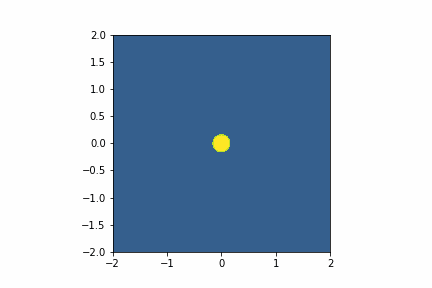
\includegraphics[width=\textwidth]{figures/no-reflector-0}
    \caption{Initial condition}
    \label{fig:no-ref-init}
  \end{subfigure}
  \begin{subfigure}[b]{0.45\textwidth}
    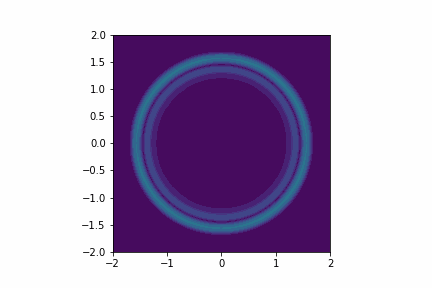
\includegraphics[width=\textwidth]{figures/no-reflector-160}
    \caption{Final $\psi$ distribution}
    \label{fig:no-ref-final}
  \end{subfigure}
  \caption{$\psi$ distribution through simulation with no reflectors}
  \label{fig:no-reflector}
\end{figure}

It is clear from figure \ref{fig:no-reflector} that the numerical solution
is behaving exactly as expected.  The initial pulse is spreading out uniformly
in the radial direction, and as such the amplitude is weakening.

\subsection{Elliptic Reflector}

We now move to using an elliptic reflector.  We wish for the beam to eminate
from one of the focci of the ellipse.  To this end we will use the following
equation for an ellipse:

$$\frac{x^2}{\alpha^2} + \frac{\left(y - \frac{\eta}{2}\right)^2}{\beta^2} = 1$$

Where $\alpha$ represents the spread in the $x$ direction, $\beta$ that of
the $y$ direction, and $\eta$ will be the distance between the two focci.
This equation forces one focci at the origin and one at the point $(0,\eta)$.

\begin{figure}[h]
  \begin{subfigure}[b]{0.45\textwidth}
    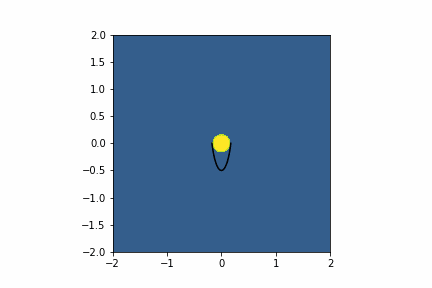
\includegraphics[width=\textwidth]{figures/elliptic-dish-0}
    \caption{Initial Condition}
    \label{fig:ellip-init}
  \end{subfigure}
  \begin{subfigure}[b]{0.45\textwidth}
    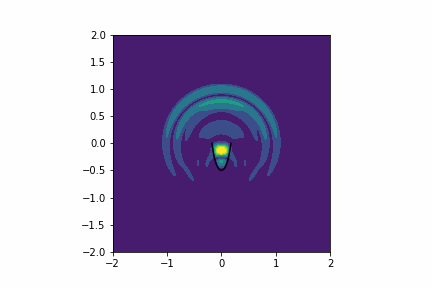
\includegraphics[width=\textwidth]{figures/elliptic-dish-100}
    \caption{$\psi$ distribution mid-simulation}
    \label{fig:ellip-mid}
  \end{subfigure}
  \begin{subfigure}[b]{0.45\textwidth}
    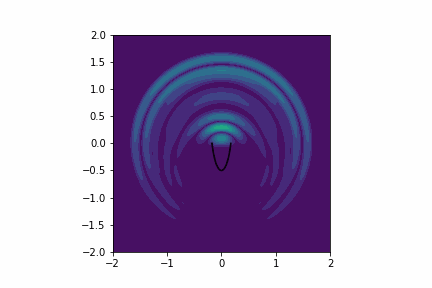
\includegraphics[width=\textwidth]{figures/elliptic-dish-160}
    \caption{$\psi$ distribution at end of simulation}
  \end{subfigure}
  \caption{$\psi$ distribution through simulation using elliptical reflector}
  \label{fig:ellip-distribution}
\end{figure}

It can be seen form figure \ref{fig:ellip-distribution} that the beam has
been pushed into the positive $y$ direction.  However there is still significant
radial spreading from the beam.

\subsection{Parabolic Reflector}

For the parabolic reflector we again want the source to be centered at the
focus of the parabola.  To this end we use the following construction of a
parabola:

$$y = \frac{x^2 - 4\lambda^2}{4\lambda}$$

This forces the focus to occur at the origin, and at $x = 0$ we have
$y = -\lambda$.

\begin{figure}[h]
  \begin{subfigure}[b]{0.45\textwidth}
    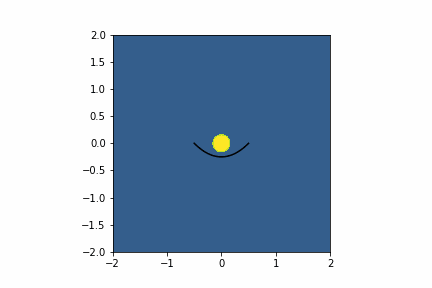
\includegraphics[width=\textwidth]{figures/parabolic-dish-0}
    \caption{Initial condition}
    \label{fig:para-init}
  \end{subfigure}
  \begin{subfigure}[b]{0.45\textwidth}
    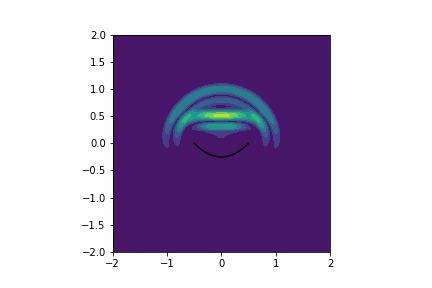
\includegraphics[width=\textwidth]{figures/parabolic-dish-100}
    \caption{Mid-simulation $\psi$ distribution}
    \label{fig:para-mid}
  \end{subfigure}
  \begin{subfigure}[b]{0.45\textwidth}
    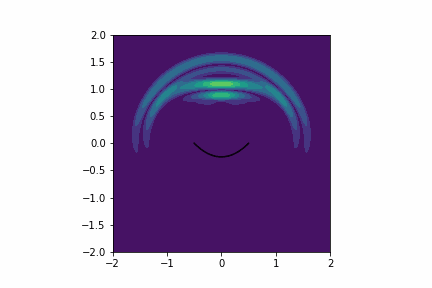
\includegraphics[width=\textwidth]{figures/parabolic-dish-160}
    \caption{Final time $\psi$ distribution}
    \label{fig:para-end}
  \end{subfigure}
  \caption{$\psi$ distribution through simulation using parabolic reflector}
  \label{fig:para-distribution}
\end{figure}

It can be seen from figure \ref{fig:para-distribution} that
the parabolic reflector nearly columnated the pulse into two distinct pulses
sent along the positive $y$-axis.  Furthermore the radial distribution of the
beam has been lessened compared to the elliptic case.


\subsection{Comparison of Beam Spreading}

Let us now compare the two antennae.  From our numerical simulations we
have an approximation for $\psi(x,y,t)$ at all spacial and temporal nodes.
We wish to look at the average distribution: $\hat{\psi}(x,y)$.  We can
construct this as follows:

\begin{equation}
  \label{eq:build-psi-avg}
  \hat{\psi}(x,y) = \frac{1}{T} \int_0^T \psi(x,y,t) \, dt \approx
  \frac{1}{T} \sum_{k=0}^N \Psi^{(k)} (\tau) = \frac{1}{N}
  \sum_{k=0}^N \Psi^{(k)}
\end{equation}

To this end we are able to generate average beam patterns for both the
elliptic and parabolic cases.

\begin{figure}[h]
  \begin{subfigure}[b]{0.49\textwidth}
    \includegraphics[width=\textwidth]{figures/elliptic-total-abs-cropped}
    \caption{Beam average for elliptic reflector}
    \label{fig:avg-elliptic}
  \end{subfigure}
  \begin{subfigure}[b]{0.49\textwidth}
    \includegraphics[width=\textwidth]{figures/parabolic-total-abs-cropped}
    \caption{Beam average for parabolic reflector}
    \label{fig:avg-parabolic}
  \end{subfigure}
  \caption{Beam averages over simulation}
  \label{fig:avg-beam-patterns}
\end{figure}

It is clear from \ref{fig:avg-beam-patterns} that the parabolic reflector is
much better at forcing the beam to proceed in the desired $y$- axis direction.
It is also clear that in both there is significant reduction in the amount
of energy sent backwards.


\section{Conclusions}

We have seen that the St\"ormer Verlet method is extremely effective for
solving the two dimensional wave equation.  Furthermore since the
finite difference approximation for the spacial derivatives, the Verlet method
works extremely well as it is also second order.

We have also seen this is
useful in examining reflections off of antennae within the plane.
From these results we were able to deduce average beam patterns and get a
glimpse into the methodology used for analyzing RADAR antennae.  In particular
using shapes based on conic sections to achieve reflections of the beams
in meaningful direction.

\newpage

\bibliography{biblio}
\bibliographystyle{ieeetr}

The numerical code used to solve this problem is located on GitHub at
\url{https://github.com/JeromeTroy/m611-project}.
In it are parameters used in the simulations to generate the figures.
\end{document}
